
\chapter{Mesurer}
\label{cp:mesurer}

Après avoir défini les objectifs et le périmètre du projet dans la phase \textit{Définir}, nous entamons désormais la phase \textit{Mesurer} de la démarche DMAIC. Cette étape consiste à quantifier l'état actuel du processus de vérification qualité, à identifier les critères de conformité critiques et à établir des indicateurs de performance mesurables.

L'objectif de cette phase est double : d'une part, collecter les données nécessaires pour évaluer l'ampleur du problème de contrôle qualité sur les surfaces CATIA, et d'autre part, formaliser les règles métier qui serviront de référence pour automatiser les vérifications. Nous nous concentrons en particulier sur les défauts surfaciques tels que les auto-intersections, qui constituent l'un des principaux obstacles à la fabricabilité des pièces conçues.

Cette partie présente les critères de qualité identifiés, leurs fondements mathématiques, ainsi que les mécanismes de détection que les macros Q-Checker métier devront automatiser.

\section{Convention de nommage}

\subsection{Contexte et enjeu}

Dans un environnement de conception collaboratif tel que CATIA~V5, chaque entité --- pièce (\textit{Part}), assemblage (\textit{Product}), surface ou feature --- est identifiée avant tout par son \textbf{nom} dans l'arbre de spécifications. Ce nom constitue la clé d'accès à l'objet pour les outils PDM/PLM (ENOVIA, Windchill), pour les scripts d'automatisation et pour l'ensemble des métiers aval (FAO, FEA, approvisionnement). Une convention de nommage est donc bien plus qu'une question d'esthétique : c'est un \textbf{contrat de lisibilité} entre tous les acteurs de la chaîne numérique.

Chez Segula Technologies, les projets automotive impliquent plusieurs centaines de pièces, développées en parallèle par des équipes réparties. En l'absence d'une règle de nommage imposée et vérifiée automatiquement, des dérives apparaissent inévitablement : noms génériques (\texttt{Part1}, \texttt{Body2}), noms en minuscules, ou noms sans code département. Ces incohérences se répercutent directement sur la chaîne de valeur.

\subsection{Justification métier}

L'absence ou le non-respect d'une convention de nommage génère des dysfonctionnements concrets à plusieurs niveaux de la chaîne de développement produit. Le \autoref{tab:impacts-nommage} synthétise les principaux impacts identifiés au cours de la phase Mesurer.

\begin{table}[H]
    \centering
    \caption{Impacts métier d'une convention de nommage non respectée}
    \label{tab:impacts-nommage}
    \begin{tabularx}{\textwidth}{|>{\bfseries\raggedright\arraybackslash}p{3.8cm}|X|}
        \hline
        \rowcolor{headerblue}
        \textcolor{white}{\textbf{Domaine impacté}} & \centering\textcolor{white}{\textbf{Conséquence opérationnelle}} \tabularnewline
        \hline
        \rowcolor{rowlight}
        Gestion de données produit (PDM/PLM) & Un nom non conforme ne remonte pas correctement dans les requêtes ENOVIA/Wind\-chill. La pièce devient introuvable dans les référentiels, générant des doublons et des risques de livraison d'une version obsolète. \\
        \hline
        \rowcolor{rowwhite}
        Assemblage & Un nom générique (\texttt{Part1}, \texttt{Body2}) rend impossible l'identification rapide d'une pièce dans un assemblage de plusieurs centaines de composants, multipliant les erreurs de substitution lors des échanges inter-équipes. \\
        \hline
        \rowcolor{rowlight}
        Automatisation Q-Checker & Les scripts de contrôle qui filtrent les pièces par code famille (ex.\ \texttt{MEC-*}, \texttt{STR-*}) échouent silencieusement si les noms ne respectent pas le format attendu. Le contrôle qualité automatisé devient inopérant sur ces pièces. \\
        \hline
        \rowcolor{rowwhite}
        Revues de conception & Un arbre de spécifications incohérent ralentit l'identification des responsabilités et des jalons de validation. Le temps perdu à identifier les pièces se répercute directement sur le planning projet. \\
        \hline
        \rowcolor{rowlight}
        Approvisionnement & Une référence non conforme rompt la traçabilité vers la nomenclature de fabrication (BOM). L'ERP ne reconnaît pas la référence, bloquant les commandes fournisseurs. \\
        \hline
    \end{tabularx}
\end{table}

\subsection{Règle de nommage retenue}

La convention adoptée pour ce projet suit le format \texttt{XXX-NNNN}, défini comme suit :

\begin{itemize}
    \item[•] \textbf{\texttt{XXX}} : exactement trois lettres majuscules, représentant le code famille ou département (\texttt{MEC} pour mécanique, \texttt{STR} pour structure, \texttt{ASS} pour assemblage, etc.).
    \item[•] \textbf{\texttt{-}} : un tiret séparateur obligatoire.
    \item[•] \textbf{\texttt{NNNN}} : trois ou quatre chiffres de séquencement, commençant à \texttt{001}.
\end{itemize}

\noindent\textbf{Exemples conformes :} \texttt{MEC-001}, \texttt{STR-0042}, \texttt{ASS-1234}.

\noindent\textbf{Exemples non conformes :} \texttt{mec-001} (minuscules), \texttt{MEC001} (tiret absent), \texttt{MEC-001A} (caractère supplémentaire non autorisé), \texttt{Part1} (nom générique CATIA par défaut).

\subsection{Typologies de non-conformités observées}

L'analyse des fichiers CAO reçus et des projets en cours a permis d'identifier quatre typologies récurrentes de non-conformité, synthétisées dans le \autoref{tab:typologies-nommage}.

\begin{table}[H]
    \centering
    \caption{Typologies de non-conformités de nommage observées}
    \label{tab:typologies-nommage}
    \begin{tabularx}{\textwidth}{|>{\bfseries\raggedright\arraybackslash}p{3.5cm}|p{3.5cm}|X|}
        \hline
        \rowcolor{headerblue}
        \textcolor{white}{\textbf{Type}} & \textcolor{white}{\textbf{Exemple}} & \centering\textcolor{white}{\textbf{Cause racine}} \tabularnewline
        \hline
        \rowcolor{rowlight}
        Nom CATIA par défaut & \texttt{Part1}, \texttt{Product2} & Pièce créée mais jamais renommée. Résultat habituel d'un travail intermédiaire non finalisé avant livraison. \\
        \hline
        \rowcolor{rowwhite}
        Casse incorrecte & \texttt{mec-001}, \texttt{Mec-001} & Absence de règle imposée dans les gabarits projet ou saisie manuelle non contrôlée. \\
        \hline
        \rowcolor{rowlight}
        Format non conforme & \texttt{MEC001}, \texttt{ME-01} & Raccourci informel pris par le concepteur (deux lettres au lieu de trois, tiret oublié). \\
        \hline
        \rowcolor{rowwhite}
        Caractères non autorisés & \texttt{MEC-001\_REV2}, \texttt{MEC-001A} & Ajout d'un indice de révision dans le nom --- pratique héritée de flux non-PLM qui contamine l'identifiant officiel. \\
        \hline
    \end{tabularx}
\end{table}

\subsection{Stratégies de correction}

La correction des non-conformités de nommage obéit à une logique de priorité selon leur impact PDM. Le \autoref{tab:correction-nommage} présente les actions correctives recommandées.

\begin{table}[H]
    \centering
    \caption{Stratégies de correction des non-conformités de nommage}
    \label{tab:correction-nommage}
    \begin{tabularx}{\textwidth}{|>{\bfseries\raggedright\arraybackslash}p{3.5cm}|X|>{\centering\arraybackslash}p{2.2cm}|}
        \hline
        \rowcolor{headerblue}
        \textcolor{white}{\textbf{Action corrective}} & \centering\textcolor{white}{\textbf{Description}} & \textcolor{white}{\textbf{Priorité}} \tabularnewline
        \hline
        \rowcolor{rowlight}
        Renommage manuel immédiat & Pour un faible nombre de pièces non conformes, le concepteur renomme directement dans l'arbre CATIA ou dans l'interface PDM en suivant le format \texttt{XXX-NNNN}. & Haute \\
        \hline
        \rowcolor{rowwhite}
        Mise à jour des gabarits & Intégrer la convention dans les \textit{templates} CATIA (\texttt{.CATPart}, \texttt{.CATProduct}) utilisés à la création de fichiers, afin que chaque nouveau fichier respecte d'emblée le format. & Haute \\
        \hline
        \rowcolor{rowlight}
        Règle de contrôle PDM & Configurer une règle de validation dans ENOVIA/Windchill qui bloque le \textit{check-in} d'un fichier au nom non conforme, faisant du PDM le dernier rempart contre les incohérences. & Moyenne \\
        \hline
        \rowcolor{rowwhite}
        Sensibilisation des équipes & Organiser une session de formation courte pour rappeler la règle de nommage, illustrée par des exemples d'impacts réels, afin de réduire les dérives à la source. & Basse \\
        \hline
    \end{tabularx}
\end{table}

\begin{block}[note]
L'automatisation de la vérification de ces règles --- via une macro Q-Checker dédiée --- sera présentée dans la phase \textit{Innover}. La phase \textit{Mesurer} se concentre ici sur la compréhension du problème et la qualification de son impact métier.
\end{block}

\iffalse
    \item[�] \textbf{Récupération du document actif :} la macro accède au document ouvert dans CATIA via \texttt{CATIA.ActiveDocument}.
    \item[�] \textbf{Identification du type de document :} distinction entre \texttt{PartDocument} (pièce) et \texttt{ProductDocument} (assemblage) à l'aide de \texttt{TypeName()}.
    \item[�] \textbf{Validation du nom (pièce) :} le nom de la pièce est extrait et comparé au pattern \texttt{\textasciicircum[A-Z]\{3\}-\textbackslash d\{3,4\}\$} via une expression régulière.
    \item[�] \textbf{Parcours récursif (assemblage) :} pour un assemblage, la macro inspecte récursivement chaque sous-produit et valide son \texttt{PartNumber}.
    \item[�] \textbf{Génération du rapport :} les noms non conformes sont collectés et affichés dans un message récapitulatif à l'utilisateur.
\fi

%% ============================================================
%%  VÉRIFICATION SOLIDE ET PLEIN
%% ============================================================
\section{Vérification qu'un Part est solide et plein}

\subsection{Définition et contexte}

Dans l'environnement CATIA~V5, un \textit{Part} est un fichier de conception (\texttt{.CATPart}) qui peut contenir deux types de géométrie :

\begin{itemize}
    \item[•] \textbf{La géométrie solide} --- créée dans le workbench \textit{Part Design}, stockée dans le \texttt{PartBody}. Elle représente un volume fermé, avec une masse et des propriétés mécaniques calculables.
    \item[•] \textbf{La géométrie surfacique} --- créée dans le workbench \textit{Generative Shape Design} (GSD), stockée dans des \texttt{HybridBody}. Elle ne définit pas de volume à elle seule.
\end{itemize}

Un Part est dit \textbf{solide et plein} lorsque son corps principal (\texttt{MainBody}) contient des features opérationnelles dont le résultat cumulé produit un \textbf{volume strictement positif}. Un volume nul signifie que les opérations booléennes (ajouts, soustractions) se sont intégralement annulées, ou qu'aucune feature solide n'a été créée.

\subsection{Justification métier}

La vérification du volume n'est pas une simple formalité géométrique. Elle répond à des exigences concrètes dans un contexte industriel, synthétisées dans le \autoref{tab:justif-volume}.

\begin{table}[H]
    \centering
    \caption{Justification métier de la vérification volumique}
    \label{tab:justif-volume}
    \begin{tabularx}{\textwidth}{|>{\bfseries\raggedright\arraybackslash}p{3.8cm}|X|}
        \hline
        \rowcolor{headerblue}
        \textcolor{white}{\textbf{Exigence}} & \centering\textcolor{white}{\textbf{Conséquence d'un volume nul ou invalide}} \tabularnewline
        \hline
        \rowcolor{rowlight}
        Fiabilité des analyses aval (CAE) & Toute simulation numérique (éléments finis, calcul thermique, mise en forme) requiert un solide fermé avec un volume défini. Un Part au volume nul génère des erreurs dans les solveurs, compromettant l'intégrité des résultats. \\
        \hline
        \rowcolor{rowwhite}
        Cohérence de la nomenclature et des calculs de masse & Dans un assemblage CATIA (\texttt{CATProduct}), la masse de chaque composant est calculée à partir de son volume et de la densité du matériau. Un Part sans volume valide fausse les calculs de masse totale, impactant les études d'équilibre, de centrage et de résistance structurelle. \\
        \hline
        \rowcolor{rowlight}
        Faisabilité fabrication & Un modèle destiné à la fabrication (usinage, fonderie, impression~3D) doit représenter un volume solide continu. Un volume nul empêche la génération correcte des trajectoires d'outil (FAO) et rend la pièce non-usinable numériquement. \\
        \hline
        \rowcolor{rowwhite}
        Automatisation et contrôle qualité & La vérification systématique du volume par macro permet de filtrer les modèles invalides \textbf{avant} leur intégration dans un assemblage ou leur transmission à un bureau de fabrication, évitant des erreurs coûteuses en phase tardive du projet. \\
        \hline
    \end{tabularx}
\end{table}

\subsection{Mécanisme de mesure dans CATIA}

\subsubsection{Le workbench SPAWorkbench (Space Analysis)}

CATIA~V5 expose un workbench dédié aux mesures géométriques avancées : le \textbf{Space Analysis Workbench} (\texttt{SPAWorkbench}), accessible par macro via la méthode \texttt{GetWorkbench("SPAWorkbench")} appliquée au document actif. Ce workbench met à disposition la méthode \texttt{GetMeasurable()}, qui accepte un objet géométrique (Body, Face, Surface) et retourne un objet \texttt{Measurable} exposant les propriétés physiques calculées. Le \autoref{tab:spa-props} résume les principales propriétés disponibles.

\begin{table}[H]
    \centering
    \caption{Propriétés de mesure exposées par le SPAWorkbench}
    \label{tab:spa-props}
    \begin{tabularx}{\textwidth}{|>{\ttfamily\raggedright\arraybackslash}p{3.5cm}|X|>{\centering\arraybackslash}p{2.5cm}|}
        \hline
        \rowcolor{headerblue}
        \normalfont\textcolor{white}{\textbf{Propriété}} & \centering\textcolor{white}{\textbf{Signification}} & \textcolor{white}{\textbf{Unité SI}} \tabularnewline
        \hline
        \rowcolor{rowlight}
        .Volume & Volume total du solide & m$^{3}$ \\
        \hline
        \rowcolor{rowwhite}
        .Area & Aire totale de la surface extérieure & m$^{2}$ \\
        \hline
        \rowcolor{rowlight}
        GetCOG() & Coordonnées du centre de gravité & m \\
        \hline
    \end{tabularx}
\end{table}

\begin{block}[note]
CATIA travaille en système SI interne (mètres). Les valeurs retournées par \texttt{SPAWorkbench} doivent être converties : volume $\times 10^{9}$ pour obtenir des mm$^{3}$, aire $\times 10^{6}$ pour obtenir des mm$^{2}$.
\end{block}

\subsubsection{Mécanisme de calcul interne}

Le moteur géométrique de CATIA, basé sur le noyau \textbf{CGM} (\textit{Convergent Geometry Modeler}), calcule le volume par intégration numérique sur la représentation B-Rep (\textit{Boundary Representation}) du solide. La représentation B-Rep décrit un solide par l'ensemble de ses faces, arêtes et sommets. Pour qu'un volume soit calculable, trois conditions doivent être satisfaites :

\begin{itemize}
    \item[•] La géométrie doit être \textbf{fermée} (pas de face manquante).
    \item[•] Les normales de toutes les faces doivent pointer vers l'\textbf{extérieur} du solide.
    \item[•] Aucune \textbf{auto-intersection} ne doit exister sur les faces ou les arêtes.
\end{itemize}

Si l'une de ces conditions est violée, CATIA retourne un volume nul ou lève une erreur.

\subsection{Stratégies de correction}

Lorsque la macro détecte un volume nul ou une anomalie, plusieurs causes sont possibles. Le \autoref{tab:correction-volume} présente les cas fréquents et les actions correctives recommandées.

\begin{table}[H]
    \centering
    \caption{Stratégies de correction en cas de volume nul ou invalide}
    \label{tab:correction-volume}
    \begin{tabularx}{\textwidth}{|>{\bfseries\raggedright\arraybackslash}p{3.2cm}|p{3.8cm}|X|}
        \hline
        \rowcolor{headerblue}
        \textcolor{white}{\textbf{Cas détecté}} & \textcolor{white}{\textbf{Cause probable}} & \centering\textcolor{white}{\textbf{Action corrective}} \tabularnewline
        \hline
        \rowcolor{rowlight}
        PartBody vide & Aucune feature solide créée & Créer un Pad, Shaft ou autre feature de base dans Part Design. \\
        \hline
        \rowcolor{rowwhite}
        Volume = 0 avec features & Pocket de même dimension qu'un Pad (annulation totale) & Vérifier l'arbre de construction --- réduire la profondeur du Pocket. \\
        \hline
        \rowcolor{rowlight}
        Erreur de mesure & Géométrie invalide (auto-intersection, face ouverte) & Utiliser \textit{Analyze~$\rightarrow$ Check Geometry} pour localiser les défauts. \\
        \hline
        \rowcolor{rowwhite}
        Mauvais type de document & Fichier Product ou Drawing ouvert au lieu d'un Part & Ouvrir le fichier \texttt{.CATPart} correspondant. \\
        \hline
        \rowcolor{rowlight}
        Volume anormalement faible & Feature mal dimensionnée ou unités incorrectes & Vérifier les unités du document (\textit{Tools~$\rightarrow$ Options~$\rightarrow$ Parameters \& Measure}). \\
        \hline
    \end{tabularx}
\end{table}

\paragraph{Utiliser Check Geometry.}
L'outil \textbf{Analyze~$\rightarrow$ Check Geometry} (disponible dans Part Design et GSD) permet d'inspecter automatiquement un solide et d'identifier les faces en auto-intersection, les arêtes non-manifold (partagées par plus de deux faces) et les faces de surface nulle. Il est recommandé d'exécuter cet outil systématiquement avant toute analyse volumique par macro, afin de garantir la validité topologique du modèle.

\paragraph{Reconstruire l'arbre de features.}
Lorsqu'une annulation de volume est constatée, il est utile de \textbf{désactiver les features} une par une (clic droit $\rightarrow$ \textit{Deactivate}) pour identifier celle qui neutralise le volume. Cette approche par isolation permet un diagnostic rapide sans modifier définitivement la géométrie.

\subsection{Limites de la méthode}

\begin{itemize}
    \item[•] La macro analyse uniquement le \textbf{MainBody} (PartBody principal). Les corps secondaires (\textit{Bodies}) et les géométries surfaciques (\textit{HybridBodies}) ne sont pas pris en compte.
    \item[•] Le \texttt{SPAWorkbench} doit être disponible dans la licence CATIA active. En l'absence de ce module, la macro lèvera une erreur à l'appel de \texttt{GetWorkbench()}.
    \item[•] La précision du calcul volumique dépend de la tolérance de modélisation définie dans les options CATIA (\textit{Tools~$\rightarrow$ Options~$\rightarrow$ Shape~$\rightarrow$ General}).
\end{itemize}

\begin{block}[note]
L'implémentation de la macro de vérification volumique --- incluant le code VBA complet --- sera détaillée dans la phase \textit{Innover}. La présente section se limite à la compréhension du problème, à sa justification métier et aux stratégies de correction.
\end{block}

%% ============================================================
%%  AUTO-INTERSECTION
%% ============================================================
\section{Auto-intersection (Offset Clipping)}

%% --- Section 1 : Définition & fondements mathématiques ---
\subsection{Définition et fondements mathématiques}

L'\textbf{auto-intersection} (également appelée \textit{Offset Clipping}) est un défaut topologique qui survient lorsqu'une surface se croise elle-même dans l'espace 3D. Concrètement, deux zones distinctes de la surface viennent occuper la même position géométrique, créant une boucle de matière incohérente. Ce phénomène est couramment rencontré lors des opérations de création d'épaisseur (\textit{Thick Surface}) ou de décalage (\textit{Offset}) sur des géométries complexes telles que les congés serrés, les nervures fines ou les surfaces à forte courbure.

\paragraph{Rayon de courbure et surface décalée.}
Lors d'une opération d'\textit{Offset} ou de \textit{Thick Surface}, la surface décalée $S_d$ est obtenue en déplaçant chaque point de la surface d'origine le long de sa normale unitaire $\mathbf{n}$ :

\begin{equation*}
    S_d(u,v) = S(u,v) + d \cdot \mathbf{n}(u,v)
\end{equation*}

où $d$ est l'épaisseur (ou la distance de décalage). La validité géométrique de cette opération repose sur une condition simple : le \textbf{rayon de courbure minimal} $R_{\min}$ de la surface d'origine doit rester strictement supérieur à l'épaisseur appliquée :

\begin{equation*}
    \boxed{R_{\min} > d}
\end{equation*}

Physiquement, le rayon de courbure mesure le « degré de cambrage » local de la surface. Plus une zone est courbée, plus son rayon de courbure est petit. Lorsque l'épaisseur $d$ atteint ou dépasse $R_{\min}$, le point décalé franchit le centre de courbure : la normale s'inverse localement et la surface générée se replie sur elle-même. La topologie devient alors \textbf{Non-Manifold} --- c'est l'auto-intersection.

%% --- Section 2 : Condition d'auto-intersection ---
\subsection{Condition d'auto-intersection}

En termes simples, une surface présente une auto-intersection lorsque deux zones distinctes de cette surface se retrouvent au même endroit dans l'espace 3D. La surface « se traverse elle-même » en formant une \textbf{courbe d'auto-intersection}. Dans le cas courant du décalage, cette situation se produit précisément lorsque $d \ge R_{\min}$ : la surface décalée se croise dans les zones de forte courbure, comme illustré dans la \autoref{fig:self_intersection}.

\begin{figure}[hbt!]
    \centering
    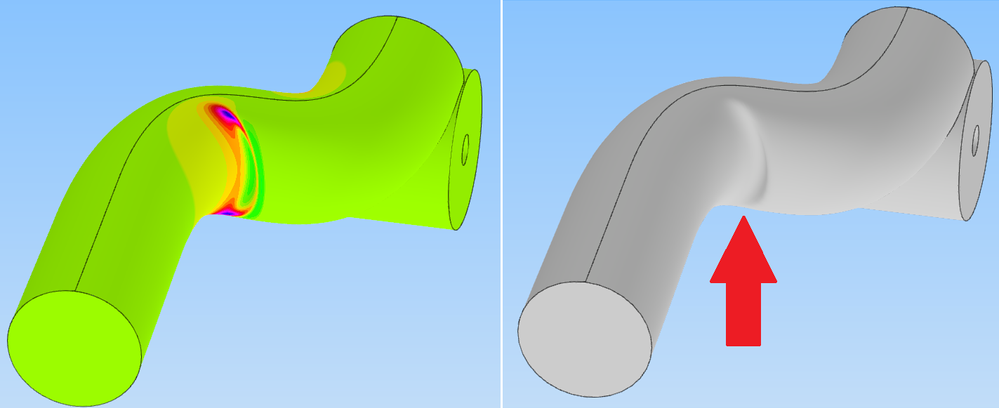
\includegraphics[width=0.45\textwidth]{Figures/self-intersection/self-intersection.png}
    \hfill
    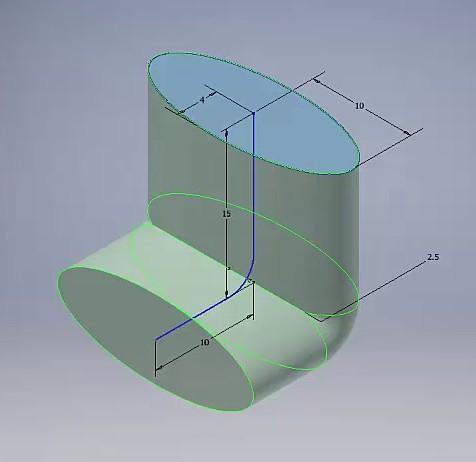
\includegraphics[width=0.45\textwidth]{Figures/self-intersection/self-intersection-2.jpg}
    \caption{Auto-intersection sur une surface décalée : la zone de forte courbure provoque un repliement de la surface sur elle-même.}
    \label{fig:self_intersection}
\end{figure}

%% --- Section 3 : Justification métier ---
\subsection{Justification métier}

Même lorsque CATIA parvient à générer la face décalée, celle-ci reste \textbf{techniquement inexploitable} par les métiers aval. La détection précoce de ce défaut est donc indispensable pour éviter des reprises coûteuses. Le \autoref{tab:impacts-auto-intersection} détaille les conséquences par domaine.

\begin{table}[H]
    \centering
    \caption{Conséquences industrielles de l'auto-intersection par domaine métier}
    \label{tab:impacts-auto-intersection}
    \begin{tabularx}{\textwidth}{|>{\bfseries\raggedright\arraybackslash}p{3.8cm}|X|}
        \hline
        \rowcolor{headerblue}
        \textcolor{white}{\textbf{Domaine}} & \centering\textcolor{white}{\textbf{Conséquence}} \tabularnewline
        \hline
        \rowcolor{rowlight}
        Fabrication assistée par ordinateur (FAO) & Les trajectoires d'outils CNC échouent ou génèrent des collisions face à une matière qui se croise elle-même. L'usinage devient imprévisible et potentiellement dangereux. \\
        \hline
        \rowcolor{rowwhite}
        Simulation par éléments finis (FEA) & Le maillage volumique ne peut pas être généré correctement sur une géométrie auto-intersectante : les éléments finis deviennent dégénérés, rendant les simulations invalides. \\
        \hline
        \rowcolor{rowlight}
        Injection plastique & Les contre-dépouilles créées par l'auto-intersection rendent le démoulage impossible sans modification de l'outillage. \\
        \hline
    \end{tabularx}
\end{table}

\begin{block}[note]
Dans l'industrie automobile, un défaut d'auto-intersection détecté tardivement --- après la livraison des outillages --- peut engendrer des coûts de reprise de plusieurs dizaines de milliers d'euros. D'où l'importance d'une détection automatisée dès la phase de conception.
\end{block}

%% --- Section 4 : Méthode de détection --- 
\subsection{Méthode de détection : la technique « Try-to-Join »}

L'API CATIA V5 ne fournit aucune fonction directe de type \texttt{Surface.IsSelfIntersecting()}. L'outil interactif \textit{Face Checker}, disponible dans le module \textit{Generative Shape Design}, permet certes de visualiser les auto-intersections, mais il n'est pas exposé dans l'API d'automatisation VBA/CATScript. Il est donc inutilisable dans une macro Q-Checker.

\paragraph{Principe de la technique.}
La solution retenue repose sur une approche indirecte baptisée \textbf{Try-to-Join}. L'idée est d'exploiter le fait que le noyau géométrique CGM de Dassault Systèmes effectue systématiquement un contrôle d'auto-intersection lors de toute opération topologique. Le principe se décompose en trois étapes :

\begin{enumerate}
    \item \textbf{Création d'un Join temporaire} --- La macro crée un objet \texttt{HybridShapeAssemble} (opération \textit{Join}) en prenant la surface cible comme unique entrée. Cette opération est ajoutée au \textit{HybridBody} du document.
    \item \textbf{Mise à jour forcée} --- L'appel à \texttt{Part.UpdateObject} déclenche le recalcul du Join par le noyau CGM. C'est à cette étape que le noyau effectue ses vérifications topologiques internes.
    \item \textbf{Capture du verdict} --- Si la surface est saine, le Join se calcule sans erreur. Si une auto-intersection est présente, le noyau CGM lève une exception que le bloc \texttt{On Error} de la macro intercepte. La surface est alors marquée comme défaillante.
\end{enumerate}

Cette technique transforme donc une \textbf{absence de fonction API} en un test fiable en s'appuyant sur les contrôles internes du noyau géométrique.

\paragraph{Avantages de l'approche.}
La technique Try-to-Join présente plusieurs atouts par rapport à une implémentation manuelle de détection :

\begin{itemize}
    \item[•] \textbf{Aucune dépendance externe :} elle utilise uniquement les objets natifs de CATIA, sans bibliothèque tierce.
    \item[•] \textbf{Fiabilité du noyau CGM :} le contrôle est délégué au même moteur géométrique que celui utilisé par les opérations de modélisation, garantissant une cohérence avec le comportement de CATIA.
    \item[•] \textbf{Simplicité d'implémentation :} quelques lignes de code VBA suffisent à mettre en place le test.
    \item[•] \textbf{Nettoyage automatique :} le Join temporaire est supprimé après le test, ne laissant aucune trace dans l'arbre de spécifications.
\end{itemize}

%% --- Section 5 : Pipeline CGM interne ---
\subsection{Pipeline interne du noyau CGM}

Pour mieux comprendre ce qui se passe « sous le capot » lors de l'appel à \texttt{Part.UpdateObject}, il est utile de décrire le pipeline de vérification exécuté par le noyau géométrique CGM (\textit{Convergence Geometric Modeler}) de Dassault Systèmes. Ce pipeline, résumé dans le \autoref{tab:etapes-cgm}, enchaîne six opérations successives allant de la discrétisation grossière jusqu'à la confirmation exacte de l'intersection.

\begin{table}[H]
    \centering
    \caption{Pipeline de vérification d'auto-intersection du noyau CGM (6 étapes)}
    \label{tab:etapes-cgm}
    \begin{tabularx}{\textwidth}{|>{\centering\arraybackslash}p{0.8cm}|>{\bfseries\raggedright\arraybackslash}p{3.2cm}|X|}
        \hline
        \rowcolor{headerblue}
        \textcolor{white}{\textbf{N°}} & \textcolor{white}{\textbf{Opération}} & \centering\textcolor{white}{\textbf{Description}} \tabularnewline
        \hline
        \rowcolor{rowlight}
        1 & Tessellation & La surface est découpée en un maillage de petits triangles. Cette approximation facettée permet de travailler avec des géométries plus simples pour les étapes suivantes. \\
        \hline
        \rowcolor{rowwhite}
        2 & Construction de l'arbre BVH & Chaque triangle est enfermé dans une boîte englobante alignée sur les axes (AABB). Ces boîtes sont organisées dans un arbre hiérarchique binaire (\textit{Bounding Volume Hierarchy}), ce qui permet de réduire la complexité des tests d'intersection de $O(n^2)$ à $O(n \log n)$. \\
        \hline
        \rowcolor{rowlight}
        3 & Test triangle--triangle & Pour chaque paire de triangles dont les boîtes englobantes se chevauchent, un test d'intersection géométrique exact est effectué. Ce test repose sur le calcul des plans supports des triangles et la vérification des intervalles de projection. \\
        \hline
        \rowcolor{rowwhite}
        4 & Filtrage des adjacences & Les paires de triangles qui partagent une arête ou un sommet sont automatiquement exclues : leur contact est un voisinage normal et non une intersection. Ce filtrage élimine les faux positifs liés à la connectivité du maillage. \\
        \hline
        \rowcolor{rowlight}
        5 & Raffinement exact & Lorsque des candidats à l'intersection subsistent après le filtrage, le noyau revient à la représentation mathématique exacte de la surface pour confirmer ou infirmer l'intersection avec une très haute précision (de l'ordre de $10^{-7}$~mm). \\
        \hline
        \rowcolor{rowwhite}
        6 & Signalement d'erreur & Si une intersection est confirmée, le noyau lève une erreur topologique. Cette erreur est propagée jusqu'à la couche VBA et capturée par le bloc \texttt{On Error} de la macro, permettant d'identifier la surface fautive. \\
        \hline
    \end{tabularx}
\end{table}

Ce pipeline illustre la stratégie « du grossier au fin » (\textit{coarse-to-fine}) adoptée par CGM : les premières étapes éliminent rapidement la majorité des zones saines grâce à des tests peu coûteux (boîtes englobantes), et seules les zones suspectes font l'objet d'un calcul exact. Cette approche garantit un bon compromis entre \textbf{performance} et \textbf{précision}.

%% --- Section 6 : Stratégies de correction ---
\subsection{Stratégies de correction}

Lorsqu'une auto-intersection est détectée par la macro, le concepteur doit intervenir sur la géométrie pour restaurer une topologie valide. Le choix de la stratégie dépend de la localisation du défaut, de la complexité de la surface et des contraintes fonctionnelles de la pièce. Le \autoref{tab:strategies-correction} présente les principales approches de correction utilisées en pratique.

\begin{table}[H]
    \centering
    \caption{Stratégies de correction d'une auto-intersection}
    \label{tab:strategies-correction}
    \begin{tabularx}{\textwidth}{|>{\bfseries\raggedright\arraybackslash}p{3.5cm}|X|>{\centering\arraybackslash}p{2.5cm}|}
        \hline
        \rowcolor{headerblue}
        \textcolor{white}{\textbf{Stratégie}} & \centering\textcolor{white}{\textbf{Description}} & \textcolor{white}{\textbf{Cas d'usage}} \tabularnewline
        \hline
        \rowcolor{rowlight}
        Augmentation du rayon de congé & Augmenter les rayons des congés (\textit{Fillets}) dans la zone de conflit afin de respecter la condition $R_{\min} > d$. C'est la correction la plus directe lorsque le défaut provient d'un congé trop serré par rapport à l'épaisseur. & Congés serrés \\
        \hline
        \rowcolor{rowwhite}
        Réduction de l'épaisseur locale & Diminuer la valeur de décalage $d$ dans la zone concernée, ou appliquer un offset variable si le cahier des charges le permet. & Épaisseur excessive \\
        \hline
        \rowcolor{rowlight}
        Healing / Lissage de courbure & Utiliser le \textit{Healing Assistant} ou l'outil \textit{Curve Smooth} de CATIA pour éliminer les micro-variations de courbure locales qui provoquent des pics de courbure sous le seuil $R_{\min}$. & Micro-défauts \\
        \hline
        \rowcolor{rowwhite}
        Découpe et reconstruction locale & Supprimer la zone de conflit et reconstruire la transition via un \textit{Multi-sections Surface}, un \textit{Blend} ou un \textit{Fill}. Cette approche offre un contrôle total sur la géométrie résultante. & Défauts localisés \\
        \hline
        \rowcolor{rowlight}
        Simplification géométrique & Remplacer une surface complexe (multi-congés, raccords G2) par une géométrie plus simple tout en respectant les tolérances fonctionnelles. & Géométries trop complexes \\
        \hline
    \end{tabularx}
\end{table}

En pratique, la correction suit une logique de \textbf{moindre modification} : on privilégie d'abord les ajustements paramétriques simples (augmentation de rayon, réduction d'épaisseur) avant de recourir à une reconstruction locale, plus lourde à mettre en œuvre et plus susceptible de modifier l'intention de conception.

%% --- Section 7 : Limites et perspectives ---
\subsection{Limites et perspectives}

\paragraph{Limites identifiées.}
Malgré son efficacité, la technique Try-to-Join présente plusieurs limites inhérentes au fonctionnement du noyau CGM et à l'environnement CATIA. Le \autoref{tab:limites-auto-intersection} en dresse la synthèse.

\begin{table}[H]
    \centering
    \caption{Limites de la détection automatisée de l'auto-intersection}
    \label{tab:limites-auto-intersection}
    \begin{tabularx}{\textwidth}{|>{\bfseries\raggedright\arraybackslash}p{3.8cm}|X|}
        \hline
        \rowcolor{headerblue}
        \textcolor{white}{\textbf{Limite}} & \centering\textcolor{white}{\textbf{Explication}} \tabularnewline
        \hline
        \rowcolor{rowlight}
        Faux négatifs & Si l'auto-intersection est d'amplitude inférieure à la tolérance interne du noyau CGM ($\approx 10^{-3}$~mm), le Join peut réussir sans détecter le défaut. La surface est alors validée à tort. \\
        \hline
        \rowcolor{rowwhite}
        Faux positifs & Une surface présentant des discontinuités de tangence marquées (raccords G0) peut faire échouer le Join sans être réellement auto-intersectante. Le défaut signalé est alors un problème de continuité, non d'auto-intersection. \\
        \hline
        \rowcolor{rowlight}
        Performance sur grands assemblages & Pour les assemblages volumineux comportant plus de 500 surfaces, la création et la suppression successives de Joins temporaires engendrent un temps de traitement significatif. \\
        \hline
        \rowcolor{rowwhite}
        Périmètre documentaire & La macro ne traite que les \texttt{CATPart}. Les documents de type \texttt{CATDrawing} et \texttt{CATAnalysis} ne sont pas pris en charge. \\
        \hline
        \rowcolor{rowlight}
        Absence de localisation précise & La technique indique \textit{qu'une} auto-intersection existe, mais ne fournit pas les coordonnées exactes de la zone de conflit. Le concepteur doit ensuite localiser visuellement le défaut. \\
        \hline
    \end{tabularx}
\end{table}

\paragraph{Perspectives d'amélioration.}
Plusieurs axes d'évolution sont envisageables pour renforcer l'outil de détection :

\begin{itemize}
    \item[•] \textbf{Coloration visuelle des défauts :} colorier automatiquement en rouge les surfaces défaillantes via \texttt{VisProperties.SetRealColor}, permettant au concepteur d'identifier instantanément les zones à corriger dans l'arbre de spécifications.
    \item[•] \textbf{Export du rapport en CSV :} générer un fichier de traçabilité contenant le nom de chaque surface, son statut (conforme / non conforme) et l'horodatage du contrôle, pour intégration dans le processus qualité du projet.
    \item[•] \textbf{Seuil de tolérance configurable :} permettre à l'utilisateur de définir la tolérance angulaire et positionnelle utilisée par le test, afin d'adapter la sensibilité de la détection au contexte métier (aéronautique vs.\ automobile, par exemple).
    \item[•] \textbf{Chaîne de contrôle intégrée :} chaîner la vérification d'auto-intersection avec les autres contrôles surfaciques (vrillage, \textit{sliver faces}, solidité) dans une macro unique, offrant un rapport qualité complet en une seule exécution.
    \item[•] \textbf{Migration vers 3DEXPERIENCE :} dans le cadre d'une future migration vers la plateforme 3DEXPERIENCE, explorer les nouvelles API de vérification géométrique qui pourraient offrir un accès direct aux fonctions de détection d'auto-intersection.
\end{itemize}

%% ============================================================
%%  VRILLAGE
%% ============================================================
\section{Vrillage (Auto-repliement)}

\subsection{Définition et fondements mathématiques}

Le vrillage (ou \textit{auto-repliement}) est une anomalie topologique majeure survenant lors de la génération de surfaces complexes via les fonctions de balayage (\textit{Sweep}) ou de surfaces multi-sections. Il se traduit par une inversion locale de la matière où la surface se croise elle-même.

Pour qu'une surface $\mathbf{S}(u,v)$ soit valide, sa paramétrisation doit être régulière. Le déterminant du Jacobien ($J$) traduit cette régularité :
\begin{equation*}
    J(u,v) = \left\| \frac{\partial \mathbf{S}}{\partial u} \times \frac{\partial \mathbf{S}}{\partial v} \right\|
\end{equation*}

\begin{itemize}
    \item[�] \textbf{Surface saine :} $J(u,v) > 0$ sur l'ensemble du domaine paramétrique.
    \item[�] \textbf{Vrillage :} apparaît lorsque $J(u,v) \le 0$. La surface perd alors sa propriété de variété (\textit{manifold}) ; les vecteurs tangents deviennent colinéaires, provoquant un effondrement géométrique.
\end{itemize}

Trois causes racines génèrent ce défaut en CAO :
\begin{itemize}
    \item[�] \textbf{Défaut de couplage :} mauvaise correspondance des points de fermeture (\textit{Closing Points}) entre sections.
    \item[�] \textbf{Conflit de tangence :} vecteurs de tangence opposés aux extrémités forçant une boucle.
    \item[�] \textbf{Saturation de l'épine (\textit{Spine}) :} rayon de courbure de la courbe guide inférieur à la demi-largeur de la section balayée.
\end{itemize}

\subsection{Justification métier : pourquoi détecter ce défaut ?}

Le vrillage constitue un critère d'exclusion lors du \textit{Q-Checking} :

\begin{itemize}
    \item[�] \textbf{Maillage (FEA) :} les solveurs ne peuvent pas traiter des faces auto-pénétrantes, entraînant un échec de simulation.
    \item[�] \textbf{Usinage (FAO) :} les normales erronées provoquent des collisions d'outil ou des trajectoires impossibles.
    \item[�] \textbf{Qualité perçue (Class A) :} rupture brutale des lignes de reflet (zébras), inacceptable en carrosserie.
\end{itemize}

La macro de détection permet d'identifier ces zones critiques avant toute transmission aux métiers aval.

\subsection{Pseudocode de l'algorithme}

% TODO : Insérer ici la capture d'écran du pseudocode / code VBA
\begin{center}
    \textit{[Image du pseudocode de la macro vrillage à insérer]}
    % \includegraphics[width=\textwidth]{Figures/pseudocode-vrillage.png}
\end{center}

\subsection{Étapes de la macro}

\begin{itemize}
    \item[�] \textbf{Discrétisation :} balayage de la surface sur une grille de points $P_{i,j}$.
    \item[�] \textbf{Calcul des normales :} extraction du vecteur unitaire $\mathbf{n}_{i,j}$ en chaque point.
    \item[�] \textbf{Test d'inversion :} si $\mathbf{n}_{i,j} \cdot \mathbf{n}_{i+1,j} < 0$, une inversion de normale est détectée.
    \item[�] \textbf{Verdict :} la zone est identifiée comme \textit{Twisted Surface} et la validation du modèle est bloquée.
\end{itemize}

% TODO : Insérer ici l'illustration visuelle des étapes de la macro
\begin{center}
    \textit{[Illustration visuelle des étapes à insérer]}
    % \includegraphics[width=\textwidth]{Figures/etapes-macro-vrillage.png}
\end{center}

\subsection{Organigramme de la macro}

% TODO : Insérer ici le flowchart de la macro vrillage
\begin{center}
    \textit{[Organigramme (flowchart) de la macro à insérer]}
    % \includegraphics[width=0.8\textwidth]{Figures/flowchart-vrillage.png}
\end{center}


